\section{复分析}

% 手稿扫描件在不在仓库里，决定是否插入图 1（目录被权限保护时也不会编译失败）
\newif\ifchainscan
\IfFileExists{images/链式法则.jpg}{\chainscantrue}{\chainscanfalse}

\subsection{Wirtinger 算子}

\begin{definition}[Wirtinger 导数]
设 $z=x+iy$。对（实）可偏导的函数 $f$，记
\[
\frac{\partial}{\partial z}=\frac12\Bigl(\frac{\partial}{\partial x}-i\frac{\partial}{\partial y}\Bigr),
\qquad
\frac{\partial}{\partial \bar z}=\frac12\Bigl(\frac{\partial}{\partial x}+i\frac{\partial}{\partial y}\Bigr).
\]
这只是\emph{记号}：只要四个一阶偏导数存在就有定义，既不要求 $f$ 全纯，也不要求 $f$ 实可微。
注意 $\dfrac1i=-i$，故 $\dfrac12\Bigl(\dfrac{\partial}{\partial x}+\dfrac1i\dfrac{\partial}{\partial y}\Bigr)$
就是 $\dfrac{\partial}{\partial z}$，不是 $\dfrac{\partial}{\partial\bar z}$。等价地，
\[
f_x=f_z+f_{\bar z},\qquad f_y=i\,(f_z-f_{\bar z}).
\]
\end{definition}

\begin{proposition}[共轭与 Wirtinger 算子]\label{prop:conj}
设 $f$ 在 $z$ 处有偏导数。则共轭恰好把两个算子互换：
\[
\overline{\frac{\partial f}{\partial z}}(z)=\frac{\partial \bar f}{\partial \bar z}(z),
\qquad
\overline{\frac{\partial f}{\partial \bar z}}(z)=\frac{\partial \bar f}{\partial z}(z),
\]
即 $\overline{\partial_z f}=\partial_{\bar z}\bar f$，$\overline{\partial_{\bar z}f}=\partial_z\bar f$。
\end{proposition}

\begin{proof}
记 $L=\dfrac{\partial f}{\partial x}(z_0)$，也就是
\[
\lim_{h\to 0,\,h\in\R}\frac{f(z_0+h)-f(z_0)}{h}=L .
\]
对实数 $h\neq0$，由共轭的定义以及 $h$ 是实数（从而 $\overline{1/h}=1/h$），
\[
\frac{\bar f(z_0+h)-\bar f(z_0)}{h}
=\frac{\overline{f(z_0+h)}-\overline{f(z_0)}}{h}
=\overline{\ \frac{f(z_0+h)-f(z_0)}{h}\ } .
\]
又共轭\emph{不改变模长}：$|\bar w-\bar L|=|\overline{w-L}|=|w-L|$。所以对任给的 $\varepsilon>0$，
\[
\left|\frac{f(z_0+h)-f(z_0)}{h}-L\right|<\varepsilon
\iff
\left|\frac{\bar f(z_0+h)-\bar f(z_0)}{h}-\bar L\right|<\varepsilon .
\]
即"$f$ 的差商趋于 $L$"与"$\bar f$ 的差商趋于 $\bar L$"的 $\varepsilon$-$\delta$ 说法\emph{逐字相同}：
使前者成立的 $\delta$ 就能使后者成立（不需要任何"极限换序"的定理，就是把定义抄一遍）。
故 $\dfrac{\partial\bar f}{\partial x}(z_0)=\bar L$；把 $h$ 换成实数 $k$ 同样得
$\dfrac{\partial\bar f}{\partial y}(z_0)=\overline{\dfrac{\partial f}{\partial y}(z_0)}$。

于是
\[
\overline{\frac{\partial f}{\partial z}}
=\overline{\frac12\Bigl(\frac{\partial f}{\partial x}-i\frac{\partial f}{\partial y}\Bigr)}
=\frac12\Bigl(\overline{\frac{\partial f}{\partial x}}+i\,\overline{\frac{\partial f}{\partial y}}\Bigr)
=\frac12\Bigl(\frac{\partial\bar f}{\partial x}+i\frac{\partial\bar f}{\partial y}\Bigr)
=\frac{\partial\bar f}{\partial\bar z},
\]
（第二步用了 $\overline{-i\lambda}=+i\bar\lambda$），第二式同理：
\[
\overline{\frac{\partial f}{\partial \bar z}}
=\frac12\Bigl(\frac{\partial\bar f}{\partial x}-i\frac{\partial\bar f}{\partial y}\Bigr)
=\frac{\partial\bar f}{\partial z}.
\]
一句话：共轭只把定义式里的 $i$ 翻成 $-i$，而 $\partial_{\bar z}$ 的定义相对于 $\partial_z$ 正好是 $i$ 变号，
所以两个算子互换名字。
（若已知"连续映射与极限可交换"（命题 \ref{prop:limit-composition}），这两步就是一句话：
共轭连续，故与极限交换，$\overline{\partial_x f}=\partial_x\bar f$；上面写的 $\varepsilon$-$\delta$ 就是不引用该命题时的做法。）
\end{proof}

\noindent
写成坐标也可核对：$f=u+iv$，$\bar f=u-iv$，则
$\dfrac{\partial\bar f}{\partial\bar z}=\frac12\bigl[(u_x+v_y)+i(u_y-v_x)\bigr]$，
而 $\overline{\dfrac{\partial f}{\partial z}}=\frac12\bigl[(u_x+v_y)-i(v_x-u_y)\bigr]$，两者相同。

\smallskip
\noindent
特别地，若 $f$ 在 $z$ 处复可导（即 $f_{\bar z}(z)=0$），则
$\dfrac{\partial\bar f}{\partial z}(z)=0$ 而 $\dfrac{\partial\bar f}{\partial\bar z}(z)=\overline{f'(z)}$：
$\bar f$ 只"依赖 $\bar z$"（反全纯）。

\subsection{补充：可微、矩阵与线性映射}

这一小节把后文反复用到的概念从头讲清楚（命题 \ref{prop:pointwise}、定理 \ref{thm:chain-general} 都依赖它们）。
顺序是"由具体到抽象、再回到具体"：

\begin{enumerate}[label=\arabic*., leftmargin=1.9em]
\item 复数怎么变成矩阵；二元函数的"微分"本来就是矩阵；
\item 一般线性映射的定义（那两个字母可以是任何"向量"）；
\item $\C$ 上实线性映射的标准形 $L(h)=Ah+B\bar h$，以及"复线性 $\iff B=0$"；
\item 实可微（它就是数分里的"二元可微"）的两种写法；
\item 回到矩阵：Cauchy--Riemann 方程的几何含义；
\item 与矩阵环 $M_n(K)$ 的联系；
\item 两条工具：极限换序；
\item 术语与符号约定（"相似"的两套意思、几个常用箭头）。
\end{enumerate}

\subsubsection*{1. 复数、列向量与矩阵}

\noindent\textbf{(a) 复数 $\to$ 矩阵。}
固定 $\lambda=a+ib\in\C$。"乘 $\lambda$"是 $\C$ 上的一个映射 $h\mapsto\lambda h$；
把它写成 $\R^2$ 上的矩阵，用的是"两列 $=$ 两个基向量的像"这条算法：
\[
\lambda\cdot 1=\lambda=a+ib\ \Longrightarrow\ \text{第 1 列}=\binom{a}{b},
\qquad
\lambda\cdot i=i\lambda=-b+ia\ \Longrightarrow\ \text{第 2 列}=\binom{-b}{a},
\]
所以
\[
\lambda=a+ib\ \longmapsto\ M_\lambda=\begin{pmatrix} a & -b\\ b & a\end{pmatrix}.
\]
验算它确实就是"乘 $\lambda$"：对 $h=x+iy$，
$M_\lambda\binom{x}{y}=\binom{ax-by}{bx+ay}$，而 $\lambda h=(a+ib)(x+iy)=(ax-by)+i(bx+ay)$，一致。

这个对应还保持运算（逐项验证即可）：
\[
M_{\lambda+\mu}=M_\lambda+M_\mu,\qquad
M_{\lambda\mu}=M_\lambda M_\mu,\qquad
M_1=I .
\]
特别地，$i\longmapsto J=\begin{pmatrix}0&-1\\ 1&0\end{pmatrix}$，而
$J^2=\begin{pmatrix}-1&0\\ 0&-1\end{pmatrix}=-I$，正好对应 $i^2=-1$。
于是 $\lambda\mapsto M_\lambda$ 是\emph{单的环同态}，像是 $M_2(\R)$ 中与 $\C$ 同构的子环
$\{aI+bJ:a,b\in\R\}$——这就是"把复数实现成实矩阵"。

\smallskip
\noindent\textbf{(b) 几何意义。} 把 $\lambda=re^{i\theta}$（$r=|\lambda|$，$\theta=\arg\lambda$）代入：
\[
M_\lambda=\begin{pmatrix} a&-b\\ b&a\end{pmatrix}
=r\begin{pmatrix}\cos\theta&-\sin\theta\\ \sin\theta&\cos\theta\end{pmatrix}=rR_\theta,
\]
即"先旋转 $\theta$，再以原点为中心放大 $r$ 倍"：圆映成圆，图形只放大不变形（保角）。
几何上这类映射叫\emph{相似变换}，所以本笔记把这种矩阵叫\textbf{旋转伸缩矩阵}
（它与高等代数里的"相似矩阵 $B=P^{-1}AP$"无关，用词撞车的问题见第 8 节）。

\smallskip
\noindent\textbf{(c) 反过来：二元函数的"微分"就是矩阵。}
设 $F=(F_1,\dots,F_m):\R^n\to\R^m$ 在 $\mathbf x_0$ 处可微，即存在 $m\times n$ 实矩阵 $J$ 使
\[
F(\mathbf x_0+\mathbf h)=F(\mathbf x_0)+J\mathbf h+o(\|\mathbf h\|)\qquad(\mathbf h\in\R^n),
\]
其中 $J\mathbf h$ 就是矩阵乘列向量。这样的 $J$ 若存在则唯一，它的元素正是偏导数：
\[
J=(J_{ij}),\qquad J_{ij}=\frac{\partial F_i}{\partial x_j}(\mathbf x_0)
\qquad\text{即：第 }j\text{ 列}=\frac{\partial F}{\partial x_j}(\mathbf x_0).
\]
读法：在定义式里取 $\mathbf h=t\mathbf e_j$（只有第 $j$ 个坐标非零）、除以 $t$ 再令 $t\to0$，
左边就是 $\partial F/\partial x_j$，右边就是 $J$ 的第 $j$ 列。
维数只有两个数字：$n=$ 自变量个数 $=$ 列数，$m=$ 函数值的分量个数 $=$ 行数。

\begin{center}
\renewcommand{\arraystretch}{1.4}
\begin{tabular}{|l|l|l|}
\hline
函数 & 微分的线性映射 & 矩阵 \\
\hline
$f:\R\to\R$（一元） & $h\mapsto f'(x_0)h$ & $1\times1$：$\bigl[\,f'(x_0)\,\bigr]$\\
\hline
$f:\R^2\to\R$（二元，一个数出） & $(h_1,h_2)\mapsto f_xh_1+f_yh_2$ & $1\times2$：$\bigl[\,f_x\ \ f_y\,\bigr]$（梯度，行向量）\\
\hline
$F=(u,v):\R^2\to\R^2$ & $\mathbf h\mapsto J\mathbf h$ & $2\times2$：$\begin{pmatrix}u_x&u_y\\v_x&v_y\end{pmatrix}$（Jacobi 矩阵）\\
\hline
\end{tabular}
\end{center}

\noindent
所以"可微"的意思就是"局部可以用一个矩阵（线性映射）逼近"。
一元时这个矩阵是 $1\times1$，也就是熟悉的导数 $f'(x_0)$——"导数就是那个线性映射"，只是平时没这么说。
复值函数 $f=u+iv:\C\to\C$ 落在表的第三行（看成 $\R^2\to\R^2$），
它的矩阵写法（复数记号）要到第 3、5 节才讲。

\subsubsection*{2. 一般的线性映射}

先把一般定义抄一遍，再把字母换成复数。

\begin{definition}[实线性映射]
设 $V,W$ 是实数域 $\R$ 上的线性空间（向量空间）。
映射 $T:V\to W$ 称为\emph{实线性}的（也记作 $\R$-线性），若对一切 $u,v\in V$ 与一切\emph{实数} $\alpha,\beta$ 都有
\[
T(\alpha u+\beta v)=\alpha T(u)+\beta T(v).
\]
本笔记主要用 $V=W=\C$ 的情形：映射 $L:\C\to\C$ 实线性，即对一切 $w_1,w_2\in\C$ 与一切实数 $\alpha,\beta$，
\[
L(\alpha w_1+\beta w_2)=\alpha L(w_1)+\beta L(w_2).
\]
若上式对一切\emph{复数} $\alpha,\beta$ 都成立，则称 $L$ 是\emph{复线性}的。
\end{definition}

\noindent
条件也可以拆成 $L(w_1+w_2)=L(w_1)+L(w_2)$ 与 $L(\alpha w)=\alpha L(w)$ 两条（合写、分写等价）。

\smallskip
\noindent
\textbf{定义里那两个字母可以是任何"向量"。} 一般情形里 $V$ 的元素长什么样都行，只要能在 $V$ 里做加法与数乘：
\begin{center}
\renewcommand{\arraystretch}{1.3}
\begin{tabular}{|l|l|l|}
\hline
向量空间 $V$ & 元素长什么样 & 线性映射的例子\\
\hline
数域 $K$ 本身 & 数 & $x\mapsto ax$\\
\hline
$K^n$ & 列向量 & $T(\mathbf x)=A\mathbf x$（$A$ 是 $m\times n$ 矩阵）\\
\hline
多项式空间 $K[t]$ & 多项式 & 求导 $D:p(t)\mapsto p'(t)$\\
\hline
连续函数空间 & 函数 & $f\mapsto\displaystyle\int_0^1 f$\\
\hline
$M_n(K)$ & 矩阵 & $X\mapsto AX-XB$\\
\hline
\end{tabular}
\end{center}

\noindent
所以"是不是线性映射"与元素是数还是列向量无关；矩阵只是"取定基之后"的坐标记录。
特别地，$T:K^n\to K^m$ 线性 $\iff$ 存在 $m\times n$ 矩阵 $A$ 使 $T(\mathbf x)=A\mathbf x$，
此时定义里的 $w_1,w_2$ 就是列向量。

\smallskip
\noindent
三个容易踩的点：
\begin{enumerate}[label=(\arabic*), leftmargin=2.2em]
\item \emph{两侧空间可以不同}：$F:\R^n\to\R^m$ 中输入的 $\mathbf h$ 是 $n$ 维列向量、输出的 $L\mathbf h$ 是 $m$ 维列向量；
$m=1$（如 $f:\R^2\to\R$）时输出就是数。
\item \emph{系数必须取自同一个域 $K$}：允许复数当系数是\emph{复}线性，只允许实数才是\emph{实}线性——
这正是后面 $\C$ 与 $M_2(\R)$ 的分界（也就是"全纯"比"实可微"强的地方）。
\item $w_1,w_2$ 只是哑变量，写成 $u,v$ 或 $\mathbf x,\mathbf y$ 都一样，
关键是"对任意两个元素、任意两个系数都成立"。
\end{enumerate}

\noindent
本例 $V=W=\C$：$\C$ 的元素是\emph{数}，但由 $\C\ni x+iy\ \longleftrightarrow\ \binom{x}{y}\in\R^2$
也可以把它们看成列向量，两种说法完全等价（就是把第 1 节的矩阵词典反过来用）。

例如 $L(w)=\lambda w$（$\lambda\in\C$）是复线性的（也是实线性的）；而 $L(w)=\bar w$、$L(w)=\operatorname{Re}w$、
$L(w)=w+\bar w$ 只是实线性的，不是复线性的（试 $\alpha=i$ 即可看出）。

\subsubsection*{3. $\C$ 上实线性映射的标准形}

\begin{proposition}[实线性映射的标准形]\label{prop:real-linear-form}
$L:\C\to\C$ 实线性 $\iff$ 存在唯一的一对 $A,B\in\C$ 使
\[
L(h)=Ah+B\bar h\qquad(h\in\C);
\]
此时
\[
A=\frac{L(1)-iL(i)}{2},\qquad B=\frac{L(1)+iL(i)}{2}.
\]
\end{proposition}

\begin{proof}
$(\Leftarrow)$ 只需验证 $L(h)=Ah+B\bar h$ 满足定义：对实数 $\alpha,\beta$，
$\overline{\alpha w_1+\beta w_2}=\alpha\bar w_1+\beta\bar w_2$，故
\[
L(\alpha w_1+\beta w_2)=A(\alpha w_1+\beta w_2)+B(\alpha\bar w_1+\beta\bar w_2)
=\alpha L(w_1)+\beta L(w_2).
\]

$(\Rightarrow)$ 写 $h=x+iy$（$x,y$ 实数）。实线性给出
\[
L(h)=L(x+iy)=xL(1)+yL(i).
\]
又 $x=\dfrac{h+\bar h}{2}$，$y=\dfrac{h-\bar h}{2i}$，代入并按 $h$ 与 $\bar h$ 归并：
\[
L(h)=\frac{L(1)-iL(i)}{2}\,h+\frac{L(1)+iL(i)}{2}\,\bar h,
\]
即 $A,B$ 如命题中所写。

唯一性：若 $Ah+B\bar h=A'h+B'\bar h$ 对一切 $h$ 成立，取 $h=1$ 得 $A+B=A'+B'$，
取 $h=i$ 得 $A-B=A'-B'$，两式相加、相减即得 $A=A'$，$B=B'$。
\end{proof}

\noindent
所以"复线性"恰是 $B=0$ 的情形（$L(h)=Ah$，就是"乘一个复数"）：
实线性映射比复线性多出一个自由参数 $B$。
（也可以直接看出：复线性时 $L(h)=L(h\cdot 1)=hL(1)$，故只能 $L(h)=\lambda h$。）
这正是全纯性在微分层面的含义——见第 4 节与命题 \ref{prop:pointwise}。

\subsubsection*{4. 实可微：就是数分里的"二元可微"}

\begin{definition}[实可微]
设 $f$ 在 $z_0$ 的某邻域内有定义。称 $f$ 在 $z_0$ 处\emph{实可微}，是指存在实线性映射 $L$ 使
\[
f(z_0+h)=f(z_0)+L(h)+o(|h|)\qquad(h\to0),
\]
其中 $o(|h|)$ 表示一个满足 $\dfrac{o(|h|)}{|h|}\to0$ 的量。由命题 \ref{prop:real-linear-form}，
这等价于：存在 $A,B\in\C$ 使
\[
f(z_0+h)=f(z_0)+Ah+B\bar h+o(|h|).
\]
\end{definition}

\noindent
按坐标写（$h=x+iy$，$L(h)=xL(1)+yL(i)$）就是数学分析里的\emph{全微分}：
\[
f(z_0+h)-f(z_0)=f_x(z_0)\,x+f_y(z_0)\,y+o(|h|),
\qquad\text{即}\qquad L(1)=f_x(z_0),\quad L(i)=f_y(z_0).
\]
后两条就是"可微 $\Rightarrow$ 偏导存在且等于微分系数"：在 $f(z_0+h)=f(z_0)+L(h)+o(|h|)$ 中取 $h=x$（实数）、
除以 $x$ 并令 $x\to0$，左边就是 $f_x(z_0)$，右边是 $L(1)$。

实可微定义中的 $L$ 若存在则唯一：设 $L_1,L_2$ 都可以，则 $(L_1-L_2)(h)=o(|h|)$；
取 $h=t\in\R$ 并除以 $t$ 得 $(L_1-L_2)(1)=0$，取 $h=it$ 得 $(L_1-L_2)(i)=0$，
再由实线性（$L(1)=L(i)=0\Rightarrow L\equiv0$）得 $L_1=L_2$。

\smallskip
\noindent
把 $z=x+iy$ 对应到 $(x,y)$、$f=u+iv$ 对应到 $(u,v)$，两边的"可微"其实就是同一件事：

\begin{center}
\renewcommand{\arraystretch}{1.45}
\begin{tabular}{|p{0.235\textwidth}|p{0.685\textwidth}|}
\hline
\textbf{数学分析：二元可微} &
$F=(u,v):\R^2\to\R^2$：存在 $2\times2$ 实矩阵 $J$ 使
$F(\mathbf x_0+\mathbf h)=F(\mathbf x_0)+J\mathbf h+o(|\mathbf h|)$，
其中 $J=\begin{pmatrix}u_x&u_y\\v_x&v_y\end{pmatrix}$（Jacobi 矩阵，$4$ 个自由度）。\\
\hline
\textbf{复分析：实可微} &
同一件事，改写成复数：存在实线性 $L$ 使 $f(z_0+h)=f(z_0)+L(h)+o(|h|)$，
且 $L(h)=f_x\,x+f_y\,y=f_z\,h+f_{\bar z}\,\bar h$；一般仍是 $4$ 个实参数。\\
\hline
\textbf{复分析：复可导} &
$\lim\limits_{h\to0}\dfrac{f(z_0+h)-f(z_0)}{h}$ 存在（$h$ 取\emph{复数}，可以用复数除法）；
等价于"实可微 $+$ 微分 $L$ 复线性"，即 $f_{\bar z}(z_0)=0$（Cauchy--Riemann 方程），
此时 $L(h)=f'(z_0)h$，只剩 $2$ 个自由度。\\
\hline
\end{tabular}
\end{center}

\noindent
这张表的第三行是第 3.3 节的命题 \ref{prop:pointwise} 要证的结论，这里先列出来做对照。
其中
\[
f_z=\tfrac12\bigl[(u_x+v_y)+i(v_x-u_y)\bigr],
\qquad
f_{\bar z}=\tfrac12\bigl[(u_x-v_y)+i(v_x+u_y)\bigr],
\]
所以 $f_{\bar z}(z_0)=0$ 恰好就是 $u_x=v_y$、$u_y=-v_x$。

\smallskip
\noindent
注意区分三档（数分里也一样）：\emph{偏导存在}最弱，推不出可微；
\emph{可微}（实可微）才有线性逼近；\emph{偏导连续}（$C^1$）是可微的常用充分条件。
第 3.3 节的注 \ref{rem:cr-needs-differentiability} 会给出"偏导存在 $+$ C-R 但不实可微"的反例。

\subsubsection*{5. 回到矩阵：复可导 $=$ 微分是旋转伸缩矩阵}

\noindent\textbf{矩阵字典（复数写法 $\leftrightarrow$ 矩阵）。}
取 $\C$ 的实基 $\{1,i\}$（即 $h=x+iy$ 对应坐标 $(x,y)$）。
线性映射的矩阵，\emph{第 $1$ 列是 $L(1)$ 的坐标，第 $2$ 列是 $L(i)$ 的坐标}：
\[
L(1)=A\cdot 1+B\cdot 1=A+B=(a+c)+i(b+d),\qquad
L(i)=Ai+B\,\bar i=i(A-B)=(d-b)+i(a-c),
\]
于是
\[
L(h)=Ah+B\bar h\ \longleftrightarrow\ \begin{pmatrix} a+c & d-b\\ b+d & a-c\end{pmatrix},
\qquad \det L=|A|^2-|B|^2 .
\]
直接验算也一样：$L(h)=(a+ib)(x+iy)+(c+id)(x-iy)
=\bigl[(a+c)x+(d-b)y\bigr]+i\bigl[(b+d)x+(a-c)y\bigr]$，比较 $x,y$ 的系数即得上面这个矩阵。
反过来从矩阵读回 $A,B$：$A=\dfrac{L(1)-iL(i)}{2}$，$B=\dfrac{L(1)+iL(i)}{2}$，即命题 \ref{prop:real-linear-form}。

\smallskip
\noindent
\emph{例。} $A=2+i$、$B=1-3i$（即 $a=2,b=1,c=1,d=-3$），则
$L\longleftrightarrow\begin{pmatrix}3&-4\\-2&1\end{pmatrix}$，$\det L=3\cdot1-(-4)(-2)=-5$；
而 $|A|^2-|B|^2=5-10=-5$，两者一致。这里 $\det L<0$，说明这个 $L$ 把定向翻转了——
一般的实线性映射允许如此（剪切、非均匀拉伸、翻转都可以）。

\smallskip
\noindent
$B=0$（复线性）时矩阵化为\emph{旋转伸缩矩阵}：若 $A=re^{i\theta}$，则
\[
L(h)=Ah\ \longleftrightarrow\ \begin{pmatrix} a & -b\\ b & a\end{pmatrix}
=r\begin{pmatrix}\cos\theta & -\sin\theta\\ \sin\theta & \cos\theta\end{pmatrix},
\qquad \det L=|A|^2=r^2>0,
\]
即"旋转 $\theta$ 再伸缩 $r$"：它把圆映成圆，因而保角。
这与第 1 节 (b) 里"乘 $\lambda$ 就是旋转加伸缩"是同一件事，只是这里 $A$ 是微分。

\smallskip
\noindent
而 $f$ 的 Jacobi 矩阵 $\begin{pmatrix}u_x&u_y\\v_x&v_y\end{pmatrix}$ 在 Cauchy--Riemann 方程成立时
恰好是这个形状（$u_x=v_y=a$，$u_y=-v_x=-b$），于是
\[
\det J=u_xv_y-u_yv_x=a^2+b^2=|f'(z_0)|^2\ \ge\ 0 .
\]
也就是说：复可导时，微分的面积伸缩因子恰是 $|f'(z_0)|^2$，而且绝不翻转定向；一般二元可微则允许 $\det J<0$。

\smallskip
\noindent
一句话：\textbf{复可导 $=$ 二元可微（实可微）$+$ 微分是复线性}。
复可导一定实可微（把 $f'(z_0)h$ 看成线性映射即可），反之不然（注 \ref{rem:cr-needs-differentiability}）。
两组式子的差别全在那个 $i$：微分允许是"任意线性变换"，还是只允许是"乘复数"。

\smallskip
\noindent
顺带说明为什么二元函数不能用"差商有极限"来定义可微：$\R^2$ 里没有"除以向量"，只能借助线性映射；
而复情形有复数除法，于是线性映射被逼成"乘一个复数"。

\subsubsection*{6. 与矩阵环 $M_n(K)$ 的联系}

高等代数里的 $M_n(K)$（$K$ 上 $n$ 阶方阵，按加法与乘法成环）在这里正好就是"线性映射全体"：
\[
\operatorname{End}_K(K^n)\longrightarrow M_n(K),\qquad \varphi\longmapsto \varphi\ \text{在标准基下的矩阵}
\]
是\emph{环同构}（保持加法、乘法与单位阵：映射的复合对应矩阵乘法）。
于是"可微 $=$ 存在线性映射"这句话，在\emph{进 $n$ 个数、出 $n$ 个数}时就可以读成"微分是 $M_n(K)$ 中的一个元素"。

$\C$ 的情形：把 $\C$ 看成二维 $\R$-向量空间，则 $\operatorname{End}_\R(\C)\cong M_2(\R)$。
"乘复数" $\lambda=a+ib$ 所对应的矩阵就是第 1 节 (a) 里的 $M_\lambda=aI+bJ$：
\[
m_\lambda\ \longleftrightarrow\ \begin{pmatrix} a & -b\\ b & a\end{pmatrix}=aI+bJ,
\qquad J=\begin{pmatrix}0&-1\\ 1&0\end{pmatrix},\quad J^2=-I,
\]
因此 $\lambda\mapsto aI+bJ$ 是单环同态，像是 $M_2(\R)$ 中同构于 $\C$ 的子环
$\C\cong\{aI+bJ:a,b\in\R\}$（$I$ 对应 $1$，$J$ 对应 $i$）。
注意 $M_2(\R)$ 非交换，而这个子环是域：交换、非零元全可逆，$\det(aI+bJ)=a^2+b^2$。

于是复分析的两句话可以这样记：
\begin{itemize}[leftmargin=1.6em]
\item \textbf{实可微}：微分 $L\in\operatorname{End}_\R(\C)\cong M_2(\R)$，可以是任意矩阵；
\item \textbf{复可导}：微分 $L$ 落在子环 $\{aI+bJ\}\cong\C$ 里（即"乘复数"），
等价于 $L(h)=Ah+B\bar h$ 中 $B=0$，等价于 Cauchy--Riemann 方程。
\end{itemize}

\noindent
对照着看：共轭 $h\mapsto\bar h$ 对应 $M_2(\R)$ 中的 $\begin{pmatrix}1&0\\0&-1\end{pmatrix}$，
它\emph{不在}子环 $\{aI+bJ\}$ 里，所以共轭不是复线性的——这就是注 \ref{rem:bar-term} 里 $\bar f$ 那一项
$\dfrac{\partial g}{\partial\bar w}\dfrac{\partial\bar f}{\partial z}$ 的代数来源。

\smallskip
\noindent
最后补一句维数："进 $n$ 个数、出 $m$ 个数"时微分属于 $M_{m\times n}(K)$，它一般\emph{不是}环
（$m\neq n$ 时乘法不封闭），只是向量空间；只有 $m=n$（如复值函数 $f=u+iv:\R^2\to\R^2$）才落回 $M_n(K)$。
例如二元的 $f:\R^2\to\R$（一个数出），微分是 $1\times2$ 的 $\bigl[\,f_x\ f_y\,\bigr]$，不是环的元素。

\subsubsection*{7. 工具：极限换序}

\begin{proposition}[复合函数的极限]\label{prop:limit-composition}
设 $\lim\limits_{h\to0}w(h)=L$，且 $F$ 在 $L$ 处连续，则 $\lim\limits_{h\to0}F\bigl(w(h)\bigr)=F(L)$。
\end{proposition}

\begin{proof}
任给 $\varepsilon>0$。由 $F$ 在 $L$ 连续，存在 $\eta>0$ 使 $|w-L|<\eta\Rightarrow|F(w)-F(L)|<\varepsilon$；
又由 $w(h)\to L$，存在 $\delta>0$ 使 $0<|h|<\delta\Rightarrow|w(h)-L|<\eta$。
于是 $0<|h|<\delta\Rightarrow|F(w(h))-F(L)|<\varepsilon$。
\end{proof}

\noindent
三个常用特例（证明就是把上式里的 $\eta$ 取成 $\varepsilon$）：
\[
F(w)=\bar w:\quad|\bar w-\bar L|=|w-L|;
\]
\[
F(w)=\operatorname{Re}w\ \text{或}\ \operatorname{Im}w:\quad|\operatorname{Re}(w-L)|\le|w-L|,\quad
|\operatorname{Im}(w-L)|\le|w-L|;
\]
\[
F(w)=|w|:\quad\bigl||w|-|L|\bigr|\le|w-L| .
\]
于是"共轭与极限可交换""取实部与极限可交换""取模与极限可交换"这类话，都是命题 \ref{prop:limit-composition} 的特例。
命题 \ref{prop:conj} 也可以用它一句话说完：共轭连续，故 $\overline{\partial_x f}=\partial_x\bar f$
（先把差商取共轭再取极限，与先取极限再取共轭，是同一件事）。

\subsubsection*{8. 术语与符号约定}

\noindent\textbf{(a) "相似矩阵"有两套意思，注意别混。}
\begin{itemize}[leftmargin=1.6em]
\item 几何上的\emph{相似变换}：旋转 $+$ 均匀伸缩，矩阵形如 $rR_\theta=\begin{pmatrix}a&-b\\ b&a\end{pmatrix}$。
本笔记一律叫它\textbf{旋转伸缩矩阵}。
\item 高等代数里的\emph{相似矩阵}：$B=P^{-1}AP$（$P$ 可逆），意思是"同一个线性变换在两组不同基下的矩阵"，
关心的是能不能对角化、有没有最简形式，与"形状是不是旋转伸缩"没有关系。
\end{itemize}

\medskip
\noindent\textbf{(b) 常用箭头。}
\begin{center}
\renewcommand{\arraystretch}{1.3}
\begin{tabular}{|c|l|p{0.52\textwidth}|}
\hline
符号 & 读法 & 意思\\
\hline
$f:X\to Y$ & 映射 & 声明 $f$ 把 $X$ 中的元素送到 $Y$ 中（定义域、值域）\\
\hline
$x\mapsto f(x)$ & 对应 & 具体元素被送到哪个元素（"送法"）\\
\hline
$L\ \longleftrightarrow\ M$ & 一一对应 & 左右是\emph{同一个对象}的两种写法（这里是同一线性映射的复数写法与矩阵写法）\\
\hline
$A\iff B$ & 当且仅当 & 命题 $A$、$B$ 互为充要条件\\
\hline
$A\Rightarrow B$ & 推出 & 由 $A$ 可推出 $B$\\
\hline
\end{tabular}
\end{center}

\noindent
最容易看错的是 $\longleftrightarrow$：它既不是"推出"也不是"等价于"，而是"词典里两边对译"。
比如 $L(h)=Ah+B\bar h\ \longleftrightarrow\ \begin{pmatrix}a+c&d-b\\ b+d&a-c\end{pmatrix}$
的意思是：左边这个映射用矩阵写出来就是右边那个矩阵，反之亦然（$A,B$ 与四个矩阵元一一对应）。

\subsection{全纯的等价刻画（Cauchy--Riemann 方程）}

\begin{proposition}[点态判据：实可微 $+$ Cauchy--Riemann 方程]\label{prop:pointwise}
设 $f$ 在 $z_0$ 实可微。则存在唯一的 $A,B\in\C$ 使
\[
f(z_0+h)=f(z_0)+Ah+B\bar h+o(|h|)\qquad (h\to 0),
\]
且 $A=\dfrac{\partial f}{\partial z}(z_0)$，$B=\dfrac{\partial f}{\partial\bar z}(z_0)$。于是
\[
f \text{ 在 } z_0 \text{ 复可导}\iff \frac{\partial f}{\partial\bar z}(z_0)=0,
\]
此时 $f'(z_0)=\dfrac{\partial f}{\partial z}(z_0)=\dfrac{\partial f}{\partial x}(z_0)$。
\end{proposition}

\begin{proof}
\emph{(1) 分解与系数。} 实可微即存在 $\R$-线性映射 $L$ 使 $f(z_0+h)=f(z_0)+L(h)+o(|h|)$。
写 $h=x+iy$，则 $L(h)=xL(1)+yL(i)$，而 $L(1)=f_x(z_0)$，$L(i)=f_y(z_0)$。
另一方面，$\C$ 上的每个 $\R$-线性映射都可唯一地写成 $L(h)=Ah+B\bar h$：由
$Ah+B\bar h=(A+B)x+i(A-B)y$ 解得
\[
A=\frac{L(1)-iL(i)}{2}=\frac{f_x(z_0)-if_y(z_0)}{2}=\frac{\partial f}{\partial z}(z_0),
\qquad
B=\frac{L(1)+iL(i)}{2}=\frac{f_x(z_0)+if_y(z_0)}{2}=\frac{\partial f}{\partial \bar z}(z_0).
\]

\emph{(2) $\Leftarrow$。} 若 $B=0$，则 $f(z_0+h)=f(z_0)+Ah+o(|h|)$，按复导数的定义，$f$ 在 $z_0$ 复可导且 $f'(z_0)=A$。

\emph{(3) $\Rightarrow$。} 若 $f$ 在 $z_0$ 复可导，则 $f(z_0+h)=f(z_0)+f'(z_0)h+o(|h|)$；
与 (1) 中的唯一分解比较得 $B=0$，$A=f'(z_0)$。
\end{proof}

\begin{proposition}[区域上：$C^1$ 版]\label{prop:region}
设 $f=u+iv$ 在区域 $D$ 内有连续偏导数。若
$\dfrac{\partial f}{\partial\bar z}\equiv0$ 于 $D$（即 $u_x=v_y,\ u_y=-v_x$ 于 $D$ 成立），
则 $f$ 在 $D$ 内全纯，且 $f'(z)=\dfrac{\partial f}{\partial z}=f_x$。
\end{proposition}

\begin{proof}
$C^1$ 蕴含每点实可微，由命题 \ref{prop:pointwise}，$f$ 在 $D$ 内每点复可导，即全纯。
\end{proof}

\begin{remark}[不能只假设"偏导存在"]\label{rem:cr-needs-differentiability}
$\dfrac{\partial f}{\partial\bar z}=0$ 单独并不足以推出全纯，"实可微"（或更强的"偏导连续"）是必须补上的条件：
\begin{enumerate}[label=(\arabic*), leftmargin=2.2em]
\item $f(z)=\dfrac{z^5}{|z|^4}\ (z\neq0)$，$f(0)=0$。此时 $f(re^{i\theta})=re^{5i\theta}$，$f$ 在原点连续；
四个偏导数在原点存在，且 $u_x(0)=v_y(0)=1$，$u_y(0)=v_x(0)=0$，Cauchy--Riemann 方程成立。
但 $\dfrac{f(z)}{z}=e^{4i\theta}$ 随方向变化，故 $f$ 在原点不实可微，更不复可导。
\item $f(z)=\exp(-z^{-4})\ (z\neq0)$，$f(0)=0$。在原点四个偏导数都存在且为 $0$，Cauchy--Riemann 方程成立，
但 $f$ 在原点甚至不连续（沿 $\arg z=\pi/8$ 有 $|f|=1$），故不可导。
\end{enumerate}
\end{remark}

\subsection{复合函数的链式法则}

先证一般情形（教材习题：只假设实可微，\emph{不}假设全纯）。

\begin{theorem}[复链式法则，Wirtinger 形式]\label{thm:chain-general}
设 $U,V$ 是 $\C$ 中的开集，$f:U\to V$ 与 $g:V\to\C$ 都只是\emph{实可微}的（作为两个实变量的函数可微），
$h=g\circ f$。则 $h$ 实可微，且对每个 $z\in U$（记 $w=f(z)$）有
\begin{align}
\frac{\partial h}{\partial z}
&=\frac{\partial g}{\partial w}(w)\cdot\frac{\partial f}{\partial z}(z)
+\frac{\partial g}{\partial \bar w}(w)\cdot\frac{\partial \bar f}{\partial z}(z),\label{eq:chain-z}\\
\frac{\partial h}{\partial \bar z}
&=\frac{\partial g}{\partial w}(w)\cdot\frac{\partial f}{\partial \bar z}(z)
+\frac{\partial g}{\partial \bar w}(w)\cdot\frac{\partial \bar f}{\partial \bar z}(z).\label{eq:chain-barz}
\end{align}
这里的 $\dfrac{\partial g}{\partial w},\dfrac{\partial g}{\partial\bar w}$ 是 $g$ 关于\emph{它自己的}变量 $w=m+in$ 的 Wirtinger 导数，
在 $w=f(z)$ 处取值；教材为省事把外层变量也写成 $z$，于是就是 $\dfrac{\partial g}{\partial z},\dfrac{\partial g}{\partial\bar z}$。
\end{theorem}

\begin{proof}[证明一（线性化，即用命题 \ref{prop:pointwise} 的分解）]
记 $A=f_z(z_0)$，$B=f_{\bar z}(z_0)$，$C=g_w(w_0)$，$D=g_{\bar w}(w_0)$，其中 $w_0=f(z_0)$。
由命题 \ref{prop:pointwise}，
\[
f(z_0+\zeta)=w_0+A\zeta+B\bar\zeta+o(|\zeta|),\qquad
g(w_0+\eta)=g(w_0)+C\eta+D\bar\eta+o(|\eta|).
\]
取 $\eta=f(z_0+\zeta)-w_0=A\zeta+B\bar\zeta+o(|\zeta|)$。则对充分小的 $\zeta$ 有 $|\eta|\le(|A|+|B|+1)|\zeta|$，
于是 $o(|\eta|)=o(|\zeta|)$（把 $\dfrac{o(|\eta|)}{|\zeta|}$ 写成 $\dfrac{o(|\eta|)}{|\eta|}\cdot\dfrac{|\eta|}{|\zeta|}$ 即见，
第一个因子趋于 $0$、第二个因子有界），且
$\bar\eta=\bar A\bar\zeta+\bar B\zeta+o(|\zeta|)$。代入得
\[
h(z_0+\zeta)-h(z_0)
=C\bigl(A\zeta+B\bar\zeta\bigr)+D\bigl(\bar B\zeta+\bar A\bar\zeta\bigr)+o(|\zeta|)
=(CA+D\bar B)\,\zeta+(CB+D\bar A)\,\bar\zeta+o(|\zeta|).
\]
这说明 $h$ 在 $z_0$ 实可微（$h(z_0+\zeta)-h(z_0)=(CA+D\bar B)\zeta+(CB+D\bar A)\bar\zeta+o(|\zeta|)$ 就是实可微定义的形式）；
按命题 \ref{prop:pointwise} 的分解唯一性（$A,B$ 由 $f_x=A+B$、$f_y=i(A-B)$ 唯一决定，故"比较系数"是合法的），
\[
\frac{\partial h}{\partial z}(z_0)=CA+D\bar B=g_wf_z+g_{\bar w}\,\overline{f_{\bar z}},
\qquad
\frac{\partial h}{\partial\bar z}(z_0)=CB+D\bar A=g_wf_{\bar z}+g_{\bar w}\,\overline{f_z}.
\]
再用命题 \ref{prop:conj}（$\overline{f_{\bar z}}=\dfrac{\partial\bar f}{\partial z}$ 与 $\overline{f_z}=\dfrac{\partial\bar f}{\partial\bar z}$）即得 \eqref{eq:chain-z}、\eqref{eq:chain-barz}。
\end{proof}

\begin{proof}[证明二（把 $h_x,h_y$ 展开，不作任何 Cauchy--Riemann 替换）]
记 $w=f(z)=m+in$，把 $g$ 看成 $(m,n)$ 的函数。由实链式法则，
\[
h_x=g_mm_x+g_nn_x,\qquad h_y=g_mm_y+g_nn_y,
\]
于是
\[
\frac{\partial h}{\partial z}=\frac12\bigl(h_x-ih_y\bigr)
=\frac12\Bigl[g_m\bigl(m_x-im_y\bigr)+g_n\bigl(n_x-in_y\bigr)\Bigr].
\]
由定义直接算（不需要任何全纯假设；记 $\bar f_z=\dfrac{\partial\bar f}{\partial z}$）：
\[
m_x-im_y=2\,\frac{\partial m}{\partial z}=\frac{\partial(f+\bar f)}{\partial z}=f_z+\bar f_z,
\qquad
n_x-in_y=2\,\frac{\partial n}{\partial z}=\frac1i\,\frac{\partial(f-\bar f)}{\partial z}=-i\,\bigl(f_z-\bar f_z\bigr),
\]
又 $g_m-ig_n=2g_w$，$g_m+ig_n=2g_{\bar w}$。代入，
\[
\frac{\partial h}{\partial z}
=\frac12\Bigl[g_m\bigl(f_z+\bar f_z\bigr)-ig_n\bigl(f_z-\bar f_z\bigr)\Bigr]
=\frac12\Bigl[(g_m-ig_n)f_z+(g_m+ig_n)\bar f_z\Bigr]
=g_wf_z+g_{\bar w}\bar f_z .
\]
同法把 $h_x+ih_y$ 展开（用 $m_x+im_y=f_{\bar z}+\bar f_{\bar z}$ 与 $n_x+in_y=-i\,(f_{\bar z}-\bar f_{\bar z})$）得
\[
\frac{\partial h}{\partial \bar z}=g_wf_{\bar z}+g_{\bar w}\bar f_{\bar z},
\]
即 \eqref{eq:chain-barz}。
\end{proof}

\begin{remark}[第二项 $\dfrac{\partial g}{\partial\bar w}\dfrac{\partial\bar f}{\partial z}$ 为什么必须在]\label{rem:bar-term}
$g$ 不假设全纯，所以它沿 $w$ 方向有两个 Wirtinger 导数 $\dfrac{\partial g}{\partial w}$ 与 $\dfrac{\partial g}{\partial\bar w}$，两者都可以非零。
复合之后，$z$ 通过两条路影响 $h$：一是 $w=f(z)$，二是 $\bar w=\bar f(z)$；而
$\dfrac{\partial\bar f}{\partial z}=\overline{\dfrac{\partial f}{\partial\bar z}}$ 一般不为零，所以第二条路有贡献，第二项丢不得。
\begin{itemize}[leftmargin=1.6em]
\item 若 $f$ 复可导（$f_{\bar z}=0$，由命题 \ref{prop:pointwise} 等价于"实可微 $+$ Cauchy--Riemann 方程"），
则 $\dfrac{\partial\bar f}{\partial z}=0$，\eqref{eq:chain-z} 变成 $\dfrac{\partial h}{\partial z}=g_wf'(z)$；
\item 若 $g$ 也复可导（$g_{\bar w}=0$），则 \eqref{eq:chain-barz} 变成
$\dfrac{\partial h}{\partial\bar z}=g_wf_{\bar z}=0$，即 $h$ 复可导且 $h'=g'(w)f'(z)$——古典链式法则（推论 \ref{cor:chain-holo}）。
\end{itemize}
只要 $f,g$ 中有一个不满足 Cauchy--Riemann 方程，两项就都要留着；这也就是 $\dfrac{\partial h}{\partial z}$ 里出现 $\bar f$ 的原因。
\end{remark}

\begin{corollary}[全纯版：古典链式法则]\label{cor:chain-holo}
设 $f$ 在 $z_0$ 复可导，$g$ 在 $w_0=f(z_0)$ 复可导，则 $h=g\circ f$ 在 $z_0$ 复可导，且
\[
h'(z_0)=g'(w_0)\,f'(z_0).
\]
特别地，全纯函数的复合仍全纯。
\end{corollary}

\begin{proof}
由命题 \ref{prop:pointwise}，$f_{\bar z}(z_0)=0$，$g_{\bar w}(w_0)=0$，从而由命题 \ref{prop:conj}，
$\dfrac{\partial\bar f}{\partial z}(z_0)=\overline{f_{\bar z}(z_0)}=0$。
代入定理 \ref{thm:chain-general} 的两式得
\[
\frac{\partial h}{\partial \bar z}(z_0)=g_wf_{\bar z}+g_{\bar w}\overline{f_z}=0,
\qquad
\frac{\partial h}{\partial z}(z_0)=g_w(w_0)f_z(z_0)=g'(w_0)f'(z_0).
\]
又 $h$ 在 $z_0$ 实可微（定理 \ref{thm:chain-general}），故由命题 \ref{prop:pointwise} 知 $h$ 在 $z_0$ 复可导且导数为上式。
\end{proof}

\begin{proof}[另证（$\varepsilon$ 函数法，不用 Wirtinger 算子）]
$g$ 在 $w_0$ 处可导。令
\[
\varepsilon(\Delta w)=
\begin{cases}
\dfrac{g(w_0+\Delta w)-g(w_0)}{\Delta w}-g'(w_0), & \Delta w\neq 0,\\[3mm]
0, & \Delta w=0,
\end{cases}
\]
则 $\lim\limits_{\Delta w\to 0}\varepsilon(\Delta w)=0$，且对\emph{一切} $\Delta w$（包括 $\Delta w=0$）都有
\[
g(w_0+\Delta w)-g(w_0)=\bigl(g'(w_0)+\varepsilon(\Delta w)\bigr)\Delta w .
\]
取 $\Delta w=f(z_0+\Delta z)-f(z_0)$。由 $f$ 在 $z_0$ 连续，$\Delta z\to0$ 时 $\Delta w\to0$，于是
\[
\frac{h(z_0+\Delta z)-h(z_0)}{\Delta z}
=\bigl(g'(w_0)+\varepsilon(\Delta w)\bigr)\cdot\frac{\Delta w}{\Delta z}.
\]
其中 $\dfrac{\Delta w}{\Delta z}\to f'(z_0)$（特别地，在 $\Delta z$ 的某去心邻域内有界），$\varepsilon(\Delta w)\to0$，
故右端趋于 $g'(w_0)f'(z_0)$，即 $h'(z_0)=g'(f(z_0))f'(z_0)$。
（这一写法自动处理了 $\Delta w=0$ 的情形，因而绕开了"$\dfrac{\Delta h}{\Delta z}=\dfrac{\Delta h}{\Delta w}\cdot\dfrac{\Delta w}{\Delta z}$ 中不能除以 $\Delta w$"的漏洞。）
\end{proof}

\begin{remark}[手稿《链式法则》与本题的差距]\label{rem:chain-ms}
\ifchainscan
手稿原稿见第 \pageref{fig:chain-ms} 页的图 \ref{fig:chain-ms}，它想证的正是定理 \ref{thm:chain-general}（教材习题）。
\else
手稿扫描件 \texttt{images/链式法则.jpg} 当前不在仓库里，故下面的图未插入；它想证的正是定理 \ref{thm:chain-general}（教材习题）。
\fi
计算路数没有错，但对不上本题的假设。
\begin{enumerate}[label=(\arabic*), leftmargin=2.2em]
\item \textbf{本题只假设实可微，用不了 Cauchy--Riemann 方程。}
手稿取算子 $\dfrac12\Bigl(\dfrac{\partial}{\partial x}+\dfrac1i\dfrac{\partial}{\partial y}\Bigr)=\dfrac{\partial}{\partial z}$
（这一步是对的，$\frac1i=-i$），随后为了消去 $\dfrac1i\dfrac{\partial h}{\partial y}$，用了
$\dfrac{\partial h}{\partial y}=i\dfrac{\partial h}{\partial x}$。
这条等式就是 Cauchy--Riemann 方程，只对全纯函数成立；本题的 $f,g$ 都只是一般实可微，完全可以不满足它，
所以这一步不能这样写。正确的做法是把 $h_y$ 老老实实算出来（证明二），或改走线性化（证明一）。
\item \textbf{少了一项。} 手稿末行得到 $\dfrac{\partial f}{\partial z}\cdot\dfrac{\partial g}{\partial z}$
（前一个因子是外层导数、后一个是内层导数），只有一项；这等于额外假设了 $g$ 全纯（$g_{\bar w}=0$）
且 $f$ 全纯（$\dfrac{\partial\bar f}{\partial z}=0$）。
一般情形里第二项 $\dfrac{\partial g}{\partial\bar w}\dfrac{\partial\bar f}{\partial z}$ 一般不为零，见注 \ref{rem:bar-term}。
\item \textbf{记号。} 外层函数的自变量是 $w=m+in$，其导数应记 $\dfrac{\partial g}{\partial w},\dfrac{\partial g}{\partial\bar w}$
并注明在 $w=f(z)$ 处取值；教材把它也写成 $\dfrac{\partial g}{\partial z},\dfrac{\partial g}{\partial\bar z}$ 是省事的写法，
手稿照抄之后与内层变量撞车。另外手稿里 $f,g,h$ 三个字母三套用法（开头 $f$ 是内层、$h$ 是外层，中段外层叫 $g$，末行外层又叫 $f$），末行因此无法解读。
建议统一记法：内层 $w=f(z)$，外层 $g(w)$，复合 $h=g\circ f$。
\end{enumerate}

\noindent
顺带：手稿中段那四行（$u_x$ 的实链式法则展开、按 $m_x,n_x$ 分组）就是证明二的骨架，本身没有错；
补上 $h_y$ 的那一半与 $\bar f$ 那一项即可。
\end{remark}

\ifchainscan
\begin{figure}[htbp]
\centering
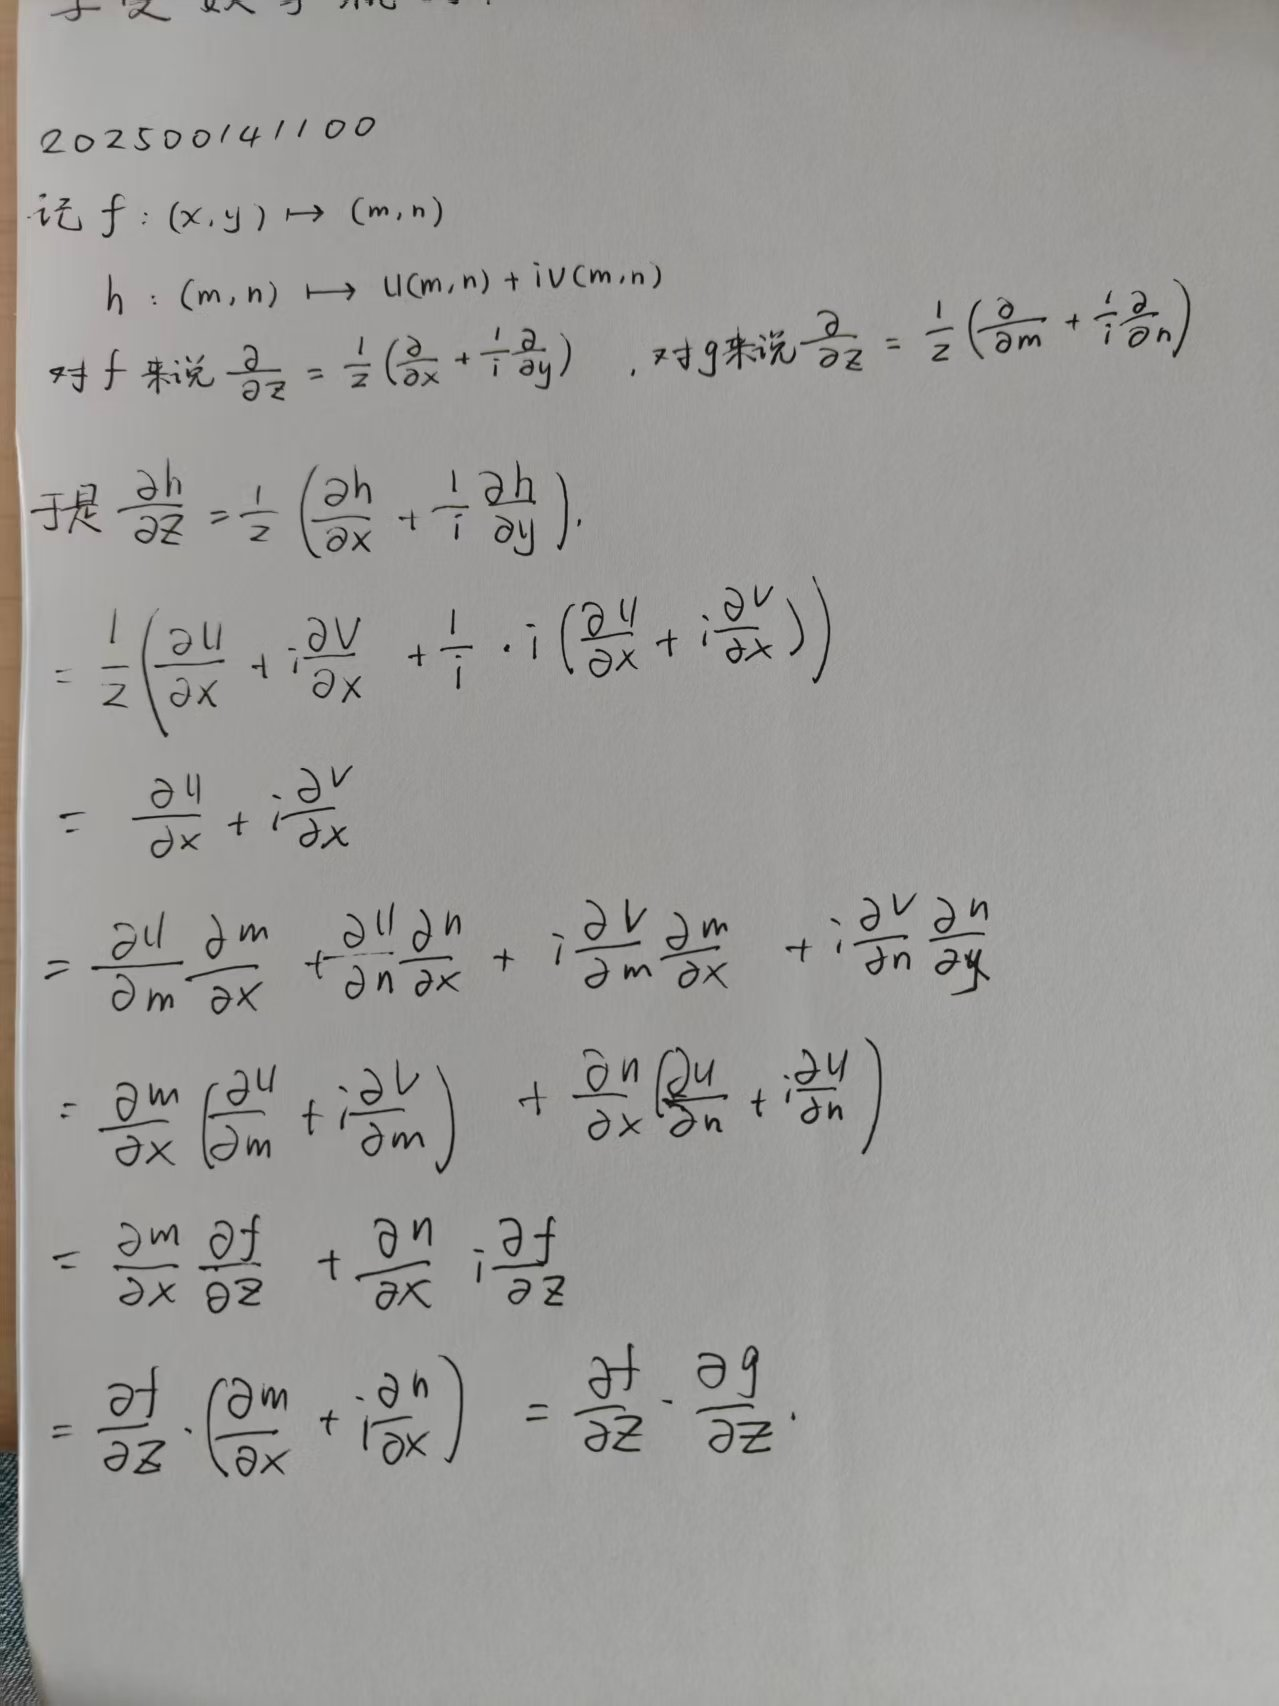
\includegraphics[width=0.42\textwidth]{images/链式法则.jpg}
\caption{手稿原稿：链式法则（2026 年 10 月 11 日）}\label{fig:chain-ms}
\end{figure}
\fi

\subsection{收敛圆周上的收敛性：$\sum z^n/n$ 在 $|z|=1$ 上除 $z=1$ 处处收敛}
\label{sec:circle-convergence}

\noindent\textbf{题目（习题 (c)）．}
证明：幂级数 $\displaystyle\sum_{n\ge1}\frac{z^n}{n}$ 在单位圆周 $|z|=1$ 上除 $z=1$ 外处处收敛。
\hfill{\small [提示：分部求和（sum by parts）。]}

\medskip
\noindent
本节按"面对这类题该从哪里想"的顺序写：先把问题定性（\S\ref{sec:circle-nature}），
再把技术骨架抽成一条与本题无关的引理（\S\ref{sec:abel-lemma}），最后回到本题（\S\ref{sec:circle-apply}）。

\subsubsection*{1. 先定性：这不是"估值"问题，是"求和"问题}
\label{sec:circle-nature}

在 $|z|<1$ 内这个级数\emph{绝对}收敛（$\sum|z|^n/n$ 收敛，用比值或根值判别法都行，收敛半径 $R=1$）。
到了收敛圆周上，"取绝对值"这条路就走到头了：$|z|=1$ 时
\[
\Bigl|\frac{z^n}{n}\Bigr|=\frac1n,
\qquad
\sum_{n\ge1}\frac1n=+\infty,
\]
所以级数在圆周上\emph{不可能}绝对收敛。更糟的是不能逐个点用 Weierstrass 判别法，
也不能在圆周上逐项积分（逐项积分要求一致收敛，而 $|z|=1$ 上一般没有一致收敛，见 \S\ref{sec:circle-apply} 注 \ref{rem:abel-nonuniform}）。

于是只剩一种可能：级数是\emph{条件收敛}的，靠"正负相消"收敛。
凡是这种局面，判断依据就不能是单项的大小 $\bigl|\frac{z^n}{n}\bigr|$，
而必须是\textbf{累积和}的大小。这一步心理转变是本题的全部难点：

\begin{center}
\emph{不研究 $\dfrac{z^n}{n}$，改研究 $A_N=z+z^2+\cdots+z^N$。}
\end{center}

$z^n$ 在圆周上绕圈，它的部分和 $A_N$ \emph{振荡但不跑远}（几何级数的部分和有闭式），
而因子 $1/n$ \emph{单调地、缓慢地}衰减。
"一个振荡有界的东西乘上一个单调衰减到 $0$ 的权重"——这类级数收敛是一条普适的定理，
而它正是用\textbf{分部求和}（Abel 求和）证明的。这就是提示里那四个字的来处。

\subsubsection*{2. 把技术骨架抽出来：一条 Abel 求和引理}
\label{sec:abel-lemma}

先在\emph{与本题无关}的一般情形下把工具磨好：一旦工具是"关于有界部分和与单调权重"的陈述，
它在别处（Fourier 级数的 Dirichlet 判别法、$\sum a_ne^{inx}$、交错级数）都能复用。
记号约定：空和为 $0$；$A_N=\sum_{n=1}^{N}c_n$。

\begin{proposition}[离散分部求和公式（Abel 变换）]\label{prop:abel-transform}
设 $\{c_n\}$、$\{w_n\}$ 是复数数列，$A_N=c_1+\cdots+c_N$（$A_0=0$）。则对 $1\le M<N$，
\begin{equation}\label{eq:abel}
\sum_{n=M}^{N}c_nw_n
=A_Nw_N-A_{M-1}w_M-\sum_{n=M}^{N-1}A_n\,(w_{n+1}-w_n).
\end{equation}
这是唯一"合适"的写法：右边只用到 $w_M,\dots,w_N$。
（若把差分方向写成 $w_n-w_{n+1}$，则不管求和补到 $N-1$ 还是 $N$ 都不再成立——
这一项的方向是"配套"的，不能单独翻。这正是本节最容易写错的一步，
所以下面证明里每一步的下标都写全。）
（$w_n\equiv1$ 时它就是 $\sum c_n=A_N$；$c_n\equiv1$ 时 $A_n=n$，于是它就是通常的分部求和
\[
\sum_{n=M}^Nw_n=Nw_N-(M-1)w_M-\sum_{n=M}^{N-1}n\,(w_{n+1}-w_n),
\]
两边同号移项即经典分部积分公式的离散版。）
\end{proposition}

\begin{proof}
\emph{（一）先证 $c_nw_n=A_nw_n-A_{n-1}w_n$。}由 $A_n=A_{n-1}+c_n$ 得
$c_n=A_n-A_{n-1}$，两边乘 $w_n$ 即得。

\emph{（二）再凑一个望远镜。}把上面这条代入并"加一项减一项"：
\[
c_nw_n=A_nw_n-A_{n-1}w_{n}=A_nw_n-A_{n-1}w_{n-1}-A_{n-1}(w_n-w_{n-1}),
\]
（右边 $=A_nw_n-A_{n-1}w_n$，因为 $-A_{n-1}w_{n-1}-A_{n-1}w_n+A_{n-1}w_{n-1}$ 相消）。
对 $n=M,\dots,N$ 求和：$\sum_{n=M}^N\bigl(A_nw_n-A_{n-1}w_{n-1}\bigr)=A_Nw_N-A_{M-1}w_{M-1}$，
于是
\[
\sum_{n=M}^Nc_nw_n=A_Nw_N-A_{M-1}w_{M-1}-\sum_{n=M}^NA_{n-1}(w_n-w_{n-1}).
\]
把右端的求和下标平移一位（$n-1\mapsto n$，即
$\sum_{n=M}^{N}A_{n-1}(w_n-w_{n-1})=\sum_{n=M-1}^{N-1}A_n(w_{n+1}-w_n)$，
其中 $n=M-1$ 那项是 $A_{M-1}(w_M-w_{M-1})$，$n=N-1$ 那项是 $A_{N-1}(w_N-w_{N-1})$）：
\[
\begin{aligned}
\sum_{n=M}^{N}c_nw_n
&=A_Nw_N-A_{M-1}w_{M-1}-A_{M-1}(w_M-w_{M-1})-\sum_{n=M}^{N-1}A_n(w_{n+1}-w_n)\\
&=A_Nw_N-A_{M-1}w_{M-1}-A_{M-1}w_M+A_{M-1}w_{M-1}-\sum_{n=M}^{N-1}A_n(w_{n+1}-w_n)\\
&=A_Nw_N-A_{M-1}w_M-\sum_{n=M}^{N-1}A_n(w_{n+1}-w_n),
\end{aligned}
\]
即 \eqref{eq:abel}。
\end{proof}

\begin{corollary}[Abel 判别法 / Dirichlet 判别法]\label{cor:dirichlet}
设 $\{c_n\}$、$\{w_n\}$ 满足：
\begin{enumerate}[label=(\roman*), leftmargin=2.4em]
\item \textbf{部分和有界}：存在 $M_0>0$，使对一切 $N$ 有 $|A_N|=\Bigl|\sum_{n=1}^Nc_n\Bigr|\le M_0$；
\item \textbf{权重单调递减趋于零}：$w_1\ge w_2\ge\cdots\ge0$ 且 $w_n\to0$；
\end{enumerate}
则 $\sum_{n\ge1}c_nw_n$ 收敛。若 $\{w_n\}$ 还只依赖于 $n$（与 $z$ 无关），
则收敛在使 (i) 中的 $M_0$ 一致的任何集合上一致。
（注意结论只是收敛：由它推不出 $\sum|c_n|w_n<\infty$，本题正是这种情形。）
\end{corollary}

\begin{proof}
用 Cauchy 判别法。对 $1\le M<N$，由 \eqref{eq:abel}（并用 $|A_{M-1}|\le M_0$、$|A_N|\le M_0$、
$w_n-w_{n+1}\ge0$、$\sum_{n=M}^{N-1}(w_n-w_{n+1})=w_M-w_N$）：
\[
\Bigl|\sum_{n=M}^{N}c_nw_n\Bigr|
\le M_0w_N+M_0w_M+M_0\,(w_M-w_N)
=2M_0w_M .
\]
右边与 $N$ 无关（$N$ 只出现在被消掉的那部分里），$M=N$ 时取空和也为 $0\le2M_0w_M$，
故对一切 $1\le M\le N$ 成立。
又 $w_M\to0$，故任给 $\varepsilon>0$，取 $M$ 充分大即得左端 $<\varepsilon$，
且这个 $M$ 只通过 $w_M$ 与 $M_0$ 起作用，与 $z$ 无关时便一致。
（若 (i) 对某个集合一致、(ii) 与参数无关，则上述 $M$ 对该集合统一，即一致收敛。）
\end{proof}

\noindent
三个伏笔：第一，证明里从来没有估计单项 $|c_nw_n|$，只用到"$A_N$ 有界"与"$w_n$ 单调"，
这正是条件收敛的典型机制；第二，结尾那个 $w_M$ 会成为本题的误差尺度；
第三，把 $w_n$ 具体取成 $1/n$ 就得到本题，下面就直接这么用。

\subsubsection*{3. 回到本题：把 $z^n$ 的部分和算出来}
\label{sec:circle-apply}

\begin{proposition}\label{prop:circle}
设 $|z|=1$，$z\ne1$。则 $\displaystyle\sum_{n\ge1}\frac{z^n}{n}$ 收敛，
并且对每个 $M\ge1$ 有 $\displaystyle\Bigl|\sum_{n=M}^{\infty}\frac{z^n}{n}\Bigr|\le\frac{4}{|1-z|\,M}$，
从而在 $\{|z|=1,\ |z-1|\ge\delta\}$ 上一致收敛。
\end{proposition}

\begin{proof}
\emph{（1）部分和的闭式。}对 $z\ne1$，由 $(1-z)(1+z+\cdots+z^{N-1})=1-z^{N}$ 得
\begin{equation}\label{eq:geom-partial}
1+z+\cdots+z^{N-1}=\frac{1-z^{N}}{1-z},
\qquad\text{故}\qquad
A_N=z+z^2+\cdots+z^{N}=\frac{z\,(1-z^{N})}{1-z},
\end{equation}
即 $A_N=\dfrac{z-z^{N+1}}{1-z}$。于是（只用 $|z|=1$）
\begin{equation}\label{eq:geom-bound}
|A_N|=\frac{|z-z^{N+1}|}{|1-z|}\le\frac{|z|+|z|^{N+1}}{|1-z|}
=\frac1{|1-z|}+\frac1{|1-z|}=\frac{2}{|1-z|}.
\end{equation}
取 $M_0=\dfrac{2}{|1-z|}$，这是与 $N$ 无关的有界量。到这一步，"$z\ne1$"这个条件终于被用上了：
$|1-z|>0$ 才能把分母除下来。

\emph{（2）套引理。}取 $c_n=z^n$（于是 $A_N$ 就是 \eqref{eq:geom-partial} 的那个），
取 $w_n=\dfrac1n$。$w_n$ 显然单调递减且趋于 $0$。
由推论 \ref{cor:dirichlet}（或直接把命题 \ref{prop:abel-transform} 用在 Cauchy 差上），级数收敛。

\emph{（3）把界算出来（顺手换一个更清楚的写法）。}用命题 \ref{prop:abel-transform}，$w_n=\frac1n$，
$w_n-w_{n+1}=\frac{1}{n}-\frac{1}{n+1}=\frac{1}{n(n+1)}$：
\[
\sum_{n=M}^{N}\frac{z^n}{n}
=\frac{A_N}{N}-\frac{A_{M-1}}{M}+\sum_{n=M}^{N-1}A_n\Bigl(\frac1n-\frac1{n+1}\Bigr),
\]
再对 $n\ge M$ 用估计 \eqref{eq:geom-bound} 中的 $|A_n|\le\dfrac{2}{|1-z|}$：
\[
\Bigl|\sum_{n=M}^{N}\frac{z^n}{n}\Bigr|
\le\frac{2}{|1-z|}\Bigl(\frac1N+\frac1M+\sum_{n=M}^{N-1}\frac{1}{n(n+1)}\Bigr)
=\frac{2}{|1-z|}\Bigl(\frac1N+\frac1M+\frac1M-\frac1N\Bigr)
=\frac{4}{|1-z|\,M},
\]
其中用了 $\sum_{n=M}^{N-1}\bigl(\frac1n-\frac1{n+1}\bigr)=\frac1M-\frac1N$。
令 $N\to\infty$ 得尾巴估计
\begin{equation}\label{eq:tail-bound}
\Bigl|\sum_{n=M}^{\infty}\frac{z^n}{n}\Bigr|\le\frac{4}{|1-z|\,M}.
\end{equation}
（误差尺度恰好是引理证明末尾那个 $w_M=1/M$，与伏笔一致。）

\emph{（4）一致收敛。}在集合 $\{|z|=1,\ |z-1|\ge\delta\}$ 上 $|1-z|\ge\delta$，
故误差 $\le\dfrac{4}{\delta M}$ 与 $z$ 无关，取 $M$ 充分大即可。
\end{proof}

\noindent
把整个解压成一句话：
\begin{center}
\emph{$z^n$ 的部分和被 $\dfrac{2}{|1-z|}$ 一致控制住，$1/n$ 单调递减趋于 $0$，
于是由 Abel（Dirichlet）判别法级数收敛；误差是 $O(1/M)$。}
\end{center}

\begin{remark}[原题为什么排除了 $z=1$，而且只排除它]\label{rem:why-z1}
两点都要交代清楚。
\begin{enumerate}[label=(\arabic*), leftmargin=2.2em]
\item \textbf{$z=1$ 处确实发散。}此时级数是调和级数 $\sum 1/n=+\infty$，
部分和 $A_N=N$ 无界，估计 \eqref{eq:geom-bound} 失效——它的右端 $\dfrac{2}{|1-z|}$ 在 $z\to1$ 时爆破，
恰好把"$1$ 是唯一坏点"这件事写在了公式里。所以这不是题目的技术性排除，而是真结论。
\item \textbf{其余点都收敛。}$|z|=1,\ z\ne1$ 时 $|1-z|$ 是正的常数，\eqref{eq:tail-bound} 给出收敛。
特别地：$z=-1$ 时级数是 $-\sum(-1)^{n-1}/n=-\ln2$，是交错调和级数，中学就见过；
$z=e^{2\pi i/3}$ 时 $1+z+z^2=0$，部分和每三步回到 $0$，有界得更明显。
\item \textbf{边界的"疏密"无关紧要。}单位圆周上的点要么就是 $1$，要么不是 $1$；
"不是 $1$"这一条与 $z$ 离 $1$ 多近无关，所以收敛是\emph{逐点}的，
整个圆周挖去一点 $|z|=1\setminus\{1\}$ 上处处收敛。但要注意下面的注 \ref{rem:abel-nonuniform}。
\end{enumerate}
\end{remark}

\begin{remark}[两个容易踩的坑]\label{rem:abel-nonuniform}
\begin{enumerate}[label=(\arabic*), leftmargin=2.2em]
\item \textbf{收敛不是一致的。}误差 \eqref{eq:tail-bound} 里的 $\dfrac{1}{|1-z|}$ 在 $z\to1$ 时无界，
故在整个 $|z|=1\setminus\{1\}$ 上\emph{不}一致收敛；
和函数 $f(z)=\sum_{n\ge1}\frac{z^n}{n}$ 在 $z\to1$ 时无界，
而一致收敛的连续函数列不可能有这样的行为。
一致收敛只在"挖掉 $1$ 的小邻域"之后成立，即 $|1-z|\ge\delta$。
\item \textbf{不能逐项积分。}圆周上 $|z|=1$，若把 $\dfrac1z$ 也乘进去做逐项积分
\[
\sum_{n\ge1}\frac1n\oint_{|z|=1}z^{n-1}\,dz ,
\]
每一步的 $\oint_{|z|=1}z^{n-1}dz=0$ 单独看没错，
但"逐项积分"需要一致收敛（本题没有），所以不能由它推出和为 $0$ 之类的结论。
这类"先积分再说"的操作在收敛圆周上是最常见的错误来源。
\item \textbf{和函数是什么（Abel 定理，此处只记结论）。}在 $|z|<1$ 内
$\sum_{n\ge1}\frac{z^n}{n}=-\log(1-z)$（把 $\frac{1}{1-z}=\sum z^n$ 逐项积分）。
由 Abel 极限定理，在 $|z|=1,\ z\ne1$ 处 $\sum_{n\ge1}\frac{z^n}{n}=-\operatorname{Log}(1-z)$
（$\operatorname{Log}$ 取主支；$z\to1$ 沿实轴时 $-\operatorname{Log}(1-z)\to+\infty$，
与 $z=1$ 处发散相容）。
\end{enumerate}
\end{remark}

\begin{remark}[条件收敛 vs.\ 绝对收敛：判断依据的替换]\label{rem:cond-vs-abs}
本题的真正教益是\textbf{条件收敛题一律先找"累积和"}。可以做成一张"触发条件 $\to$ 该想到什么"的表：

\medskip
\noindent
记 $A_N=c_1+\cdots+c_N$（\emph{累积和}，即部分和）。
\begin{enumerate}[label=(\arabic*), leftmargin=2.2em]
\item 看到 $\sum c_nw_n$，而 $|c_n|$ 不衰减（如 $|c_n|=1$）：
绝对收敛无望，改看 $A_N$——只要 $A_N$ 有界、$w_n$ 单调递减趋于 $0$，级数就收敛。
\item 看到 $c_n=z^n$、$|z|=1$：先算几何和闭式 $(1-z)A_N=?$，得到 $|A_N|\le\dfrac{2}{|1-z|}$。
\item 看到 $c_n=e^{inx}$（三角级数）：同一套，$|\sum_{n\le N}e^{inx}|\le\dfrac{1}{|\sin(x/2)|}$，
由此得 $\sum\dfrac{\cos nx}{n}$、$\sum\dfrac{\sin nx}{n}$ 的收敛（Dirichlet 判别法）。
\item 看到 $w_n$ 单调递减趋于 $0$ 而 $\sum w_n=\infty$：收敛是可能的，但只能是\emph{条件}收敛，
误差尺度通常是 $w_M$；此时不许用一致收敛的定理。
\item 想用一致收敛、逐项积分、逐项求导：先检查参数在紧集上是否\emph{远离坏点}
（本题的坏点是 $1$，好的集合是 $|1-z|\ge\delta$）。
\end{enumerate}
\end{remark}

\begin{remark}[与 Stein 教材的位置]\label{rem:stein-loc}
本题出自 Stein--Shakarchi《复分析》第 3 章"幂级数与亚纯函数"里幂级数那一节的习题
（"求和"提示所在的题组；据我记是第 16 题，其后的第 17 题要求用 Dirichlet 判别法再证一遍——
若与书上题号有出入，以书为准）。
教材把它排在"收敛半径 $=1$、边界上的收敛性必须逐点判断"的语境里，
所以本题也回答了那个语境下的自然追问：$R=1$ 时边界上到底哪些点收敛？
答案不是"收敛圆盘开、圆周不确定"这种含糊话，而是\emph{除一点外全部收敛}。
\end{remark}

\subsection{工具：上下极限的不等式链（比值法与根值法谁更强）}
\label{sec:limsup-tools}

上一小节的 $z=1$ 用了一次"$|1-z|>0$"；这一小节补另一件被反复忘掉的工具：
判断收敛半径时，比值法失败而根值法还能用的原因，
以及陈纪修《数学分析》里那条不等式链它是怎么证的、为什么好记。

\subsubsection*{1. 这条链说的是什么}

它把两个极限过程联系起来：
"相邻两项之比的极限"与"开 $n$ 次方的极限"。
在级数里，前者是比值判别法、后者是根值判别法；
在幂级数里，两者都用来算收敛半径（柯西--哈达玛）。

用一句话记住链的内容：

\begin{center}
\emph{相邻比值的上下极限，夹住了开 $n$ 次方的上下极限。}
\end{center}

它为什么该成立？两边都在量"数列的增长率"：
$\Bigl|\dfrac{a_{n+1}}{a_n}\Bigr|$ 是\emph{逐点的、相邻的}增长率，
$|a_n|^{1/n}$ 是\emph{把倍数摊平}之后的平均增长率。
比较两者用的就是"用相邻比估计远处的项"：把 $n-N$ 个不等式连乘，
再开 $n$ 次方把 $n-N$ 个因子摊到每一步上。整个证明只有这两招。

\subsubsection*{2. 四件必备的极限上下极限事实}

为了不用一遍书，把用得到的都列在这（都在 $\overline\R=[-\infty,+\infty]$ 中取值；
$a_n\ge0$）：
\begin{enumerate}[label=(F\arabic*), leftmargin=2.6em]
\item \textbf{永远存在}：$\limsup a_n$、$\liminf a_n$ 对\emph{任何}实数列都有定义，不像极限会不存在。
\item \textbf{定义式}：$\displaystyle\limsup_{n\to\infty}a_n=\lim_{N\to\infty}\Bigl(\sup_{n\ge N}a_n\Bigr)
=\inf_{N\ge1}\Bigl(\sup_{n\ge N}a_n\Bigr)$；$\liminf$ 把 $\sup$ 换成 $\inf$。
\item \textbf{集合关系}：$\liminf a_n=\inf E$、$\limsup a_n=\sup E$，其中 $E$ 是 $\{a_n\}$ 的一切收敛子列的极限之集。
\item \textbf{保序}：$a_n\le b_n$（对一切充分大的 $n$）$\Rightarrow$ $\limsup a_n\le\limsup b_n$，$\liminf a_n\le\liminf b_n$。
\item \textbf{把 $\limsup$ 当"最终上界"用}：$c>\limsup a_n$ $\Rightarrow$ 存在 $N$ 使一切 $n\ge N$ 有 $a_n<c$；
$c<\liminf a_n$ $\Rightarrow$ 存在 $N$ 使一切 $n\ge N$ 有 $a_n>c$。
（这一条是下面全部证明的唯一发动机。）
\item \textbf{与四则运算}：$\limsup(a_n+b_n)\le\limsup a_n+\limsup b_n$（一般取不到等号）；
$a_n\ge0$ 时 $\limsup(a_nb_n)\le\bigl(\limsup a_n\bigr)\bigl(\limsup b_n\bigr)$。
\item \textbf{常数不改变}：$c>0$ 时 $\limsup(ca_n)=c\limsup a_n$；$\lim_{n}(a_n)^{1/n}=1$（$a_n\to a>0$ 时）。
\item \textbf{夹在中间}：$\liminf a_n\le\limsup a_n$；两者相等（有限或同为 $\pm\infty$）$\iff$ 极限存在且等于它。
\end{enumerate}

\begin{proposition}[上下极限不等式链]\label{prop:limsup-chain}
设 $a_n>0$（$n\ge1$）。记
\[
L=\liminf_{n\to\infty}\frac{a_{n+1}}{a_n},\qquad
\sigma=\limsup_{n\to\infty}\frac{a_{n+1}}{a_n},\qquad
\ell=\liminf_{n\to\infty}a_n^{1/n},\qquad
\tau=\limsup_{n\to\infty}a_n^{1/n}.
\]
则
\begin{equation}\label{eq:limsup-chain}
L\ \le\ \ell\ \le\ \tau\ \le\ \sigma .
\end{equation}
更具体地：链的\emph{左半}是 $L\le\ell$，\emph{右半}是 $\tau\le\sigma$；
中间的 $\ell\le\tau$ 只是 (F8)。
\end{proposition}

\begin{proof}
\textbf{预备（为什么只要证两半）。}
由 (F8) 立刻有 $\ell\le\tau$；于是剩下 $L\le\ell$ 与 $\tau\le\sigma$ 两半。
两半的证明是同一个套路，但\textbf{不等式方向的处理方式不同}，所以分开写清楚。
（两者都可以看成 (F5) 的直接后果，共同点是把"对某个 $c$ 的最终估计"变成"对 $L,\sigma$ 的估计"。）

\medskip
\noindent\textbf{右半 $\tau\le\sigma$。}
设 $c$ 是 $\sigma$ 的任一严格上界，即 $c>\sigma=\limsup_n\frac{a_{n+1}}{a_n}$。
由 (F5)，存在 $N$ 使
\[
\frac{a_{n+1}}{a_n}\le c\qquad(n\ge N).
\]
\textbf{把 $n-N$ 个不等式连乘}：对 $n>N$，
\[
a_n=\frac{a_n}{a_{n-1}}\cdot\frac{a_{n-1}}{a_{n-2}}\cdots\frac{a_{N+1}}{a_N}\cdot a_N\le a_N\,c^{\,n-N}.
\]
\textbf{开 $n$ 次方把因子摊平}：
\[
a_n^{1/n}\le a_N^{1/n}\,c^{\,1-N/n}=c\cdot\underbrace{a_N^{1/n}}_{\to1}\cdot\underbrace{c^{-N/n}}_{\to1}.
\]
由 (F4)（保序）与 (F7)（乘常数、常数开方），
\[
\tau=\limsup_{n\to\infty}a_n^{1/n}
\le\lim_{n\to\infty}\Bigl(c\,a_N^{1/n}c^{-N/n}\Bigr)=c .
\]
这对一切 $c>\sigma$ 成立，令 $c\downarrow\sigma$（即对一切 $\sigma$ 的严格上界取下确界）得 $\tau\le\sigma$。

\medskip
\noindent\textbf{左半 $L\le\ell$。}
这里要证下极限的不等式，用 (F5) 的"另一半"：设 $c$ 满足 $0<c<L=\liminf_n\frac{a_{n+1}}{a_n}$，
则存在 $N$ 使
\[
\frac{a_{n+1}}{a_n}\ge c\qquad(n\ge N).
\]
连乘得 $a_n\ge a_Nc^{\,n-N}$，开 $n$ 次方得
\[
a_n^{1/n}\ge c\cdot a_N^{1/n}c^{-N/n}\ \xrightarrow[n\to\infty]{}\ c ,
\]
于是 $\ell=\liminf_n a_n^{1/n}\ge c$（用 (F4) 的 $\liminf$ 版本；这里用的是 $c$ 是\emph{下}界这件事，
与右半用 $c$ 是\emph{上}界是两处不同的假设，不能一句话带过）。
对一切 $c<L$ 成立，故 $\ell\ge L$，即 $L\le\ell$。
\end{proof}

\begin{remark}[为什么这里想得到、记不住也推得出]\label{rem:why-chain}
三个可复用的"想头"：
\begin{enumerate}[label=(\arabic*), leftmargin=2.2em]
\item \textbf{把"最终估计"当成唯一的工具。}
$\limsup$ 的定义就是为了让 (F5) 成立：想控制 $\limsup$ 就取一个严格大的 $c$ 做最终上界，
想控制 $\liminf$ 就取一个严格小的 $c$ 做最终下界。见到上下极限先想这一条。
\item \textbf{逐项连乘}:相邻比值的作用是"接着走一步"。
要把它变成对 $a_n$ 的估计，唯一的办法是连乘 $\dfrac{a_{n}}{a_{n-1}}\cdots\dfrac{a_{N+1}}{a_N}$。
\item \textbf{开 $n$ 次方是"摊平"}:$c^{\,n-N}$ 里的 $n-N$ 是"乘了 $n-N$ 次"，
一旦开 $n$ 次方，威力就变成 $c^{1-N/n}\to c$ 和一个趋 $1$ 的修正因子。
取对数看更透明：$q_n=\frac{a_{n+1}}{a_n}$，$p_n=\ln q_n$ 时
\[
\ln a_n^{1/n}=\frac{1}{n}\sum_{k=1}^{n}p_k+O\Bigl(\frac1n\Bigr)
\]
就是"前缀算术平均"，而"前缀平均的上下极限夹在 $p_k$ 的上下极限之间"是算术平均的常识
（陈纪修书里证这条时用"先斩后奏"取对数，讲的就是这件事）。上述连乘 + 开方就是它的"不打对数"版本。
\end{enumerate}
\end{remark}

\begin{remark}[判别法之间的关系：根值法严格强于比值法]\label{rem:root-vs-ratio}
对幂级数 $\sum a_nz^n$，柯西--哈达玛公式说（$0\le R\le+\infty$）
\[
\frac1R=\limsup_{n\to\infty}|a_n|^{1/n},
\]
（约定 $\frac10=+\infty$、$\frac1{+\infty}=0$；$R$ 就是收敛半径）。
而链 \eqref{eq:limsup-chain} 表明，只要 $\lim\bigl|\frac{a_{n+1}}{a_n}\bigr|$ 存在，它就等于 $\limsup|a_n|^{1/n}$，
于是\textbf{比值判别法是根值判别法的特例}；反过来不成立：

\begin{example}\label{ex:ratio-fails}
取 $a_n=2^{\,n+(-1)^n}$（即 $a_{2k}=2^{2k+1}$、$a_{2k+1}=2^{2k}$），则
\[
\frac{a_{n+1}}{a_n}=
\begin{cases}
2^{-2} & n\ \text{偶},\\[2pt]
2^{+2} & n\ \text{奇},
\end{cases}
\]
故 $\sigma=4$、$L=\frac14$，链 \eqref{eq:limsup-chain} 在 $\tau$ 上留出了空隙的余地：实际算得
\[
a_n^{1/n}=2^{\,1+(-1)^n/n}\ \longrightarrow\ 2,
\qquad\text{所以}\qquad
\frac1R=2,\qquad R=\frac12 .
\]
根值法给出 $R=\frac12$；比值法只能说"$\frac14\le\frac1R\le4$"，
连 $\sum a_nz^n$ 在 $|z|<\frac12$ 内收敛都推不出来——这就是"比值法失败、根值法照样能用"的最简例子。
\end{example}
（同一个意思的另一种说法：若 $\{a_n\}$ 的符号频繁变化，$\frac{a_{n+1}}{a_n}$ 会被"变号"搅乱，
而 $|a_n|^{1/n}$ 把变号"压掉了"，所以后者更稳。）

\end{remark}
